\section{Background}
\label{sec:back}

This background is drawn from the research task C, where the problem of using and implementing Sum Product networks are discussed in details.

A \emph{join probability distribution} (JPD) can be written as a polynomial.
Indeed, \cite{Darwiche2009} proposed a novel way of representing the JPD represented by a \emph{Bayesian network} (BN) as a simple polynomial, called a \emph{network polynomial}.
Given a JPD, it is added to each configuration (row) of it variables called indicators.
Each variable in a JPD has a correspondent indicator.
This type of variables can only assume values zeros or ones.
They are used to mark the correspondent JPD variable as being used or not.
Next, the polynomial network can be obtained by summing each row of the JPD.


\begin{example}
Consider the BN in Figure \ref{fig:bn}.
By definition \citep{Koller:2009wk}, the JPD represented by the BN can be obtained by multiplying all conditional probability tables (CPTs).
Figure \ref{fig:jpd} shows the JPD represented by the BN in Figure \ref{fig:bn}.
Now, the indicator variables can be added, being one per variables in the JPD.
Figure \ref{fig:jpd_ind} illustrated the JPD with indicator variables $\lambda_x$ for each JPD variable $x$.
One can now represent the JPD by summing all terms for each row of the table.
The polynomial network representing the JPD in Figure \ref{fig:jpd_ind} is:
\begin{eqnarray}
    f ~&=&~ \lambda_a \lambda_b \theta_a \theta_{b|a}
    + \lambda_a \lambda_{\overline{b}} \theta_a \theta_{\overline{b}|a}
    + \lambda_{\overline{a}} \lambda_b \theta_{\overline{a}} \theta_{b|\overline{a}}
    + \lambda_{\overline{a}} \lambda_{\overline{b}} \theta_{\overline{a}} \theta_{\overline{b}|\overline{a}}, \label{eq:np}
\end{eqnarray}
where each variable $A$ and $B$ can assume values in $\{a, \overline{a}\}$ and $\{b, \overline{b}\}$, respectively.
\end{example}

\begin{figure}[hbt]
    \begin{center}
    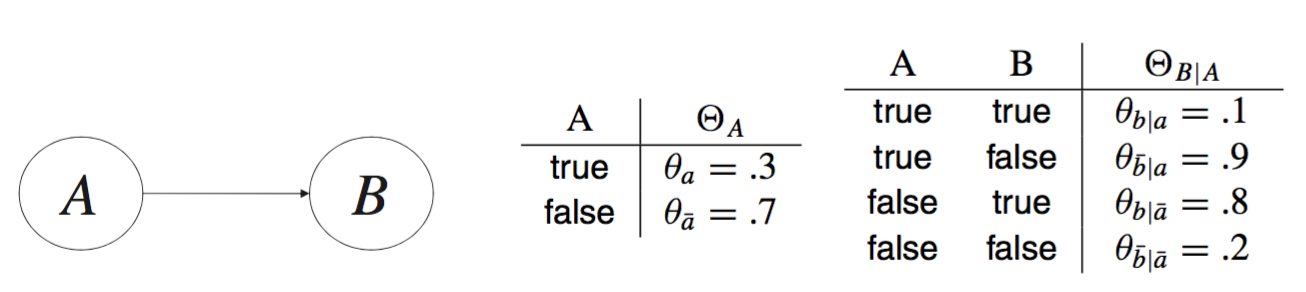
\includegraphics[width=\textwidth]{figures/bn.png}
    \caption{A BN defined by a DAG and a set of CPTs.}
    \label{fig:bn}
    \end{center}
\end{figure}

\begin{figure}[hbt]
    \begin{center}
    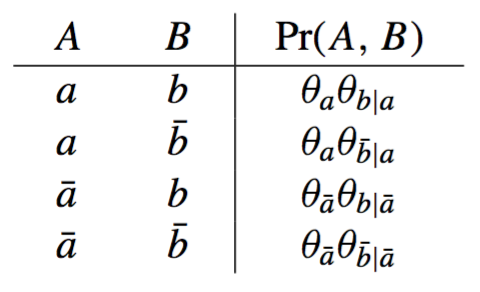
\includegraphics[width=0.35\textwidth]{figures/jpd.png}
    \caption{A JPD represented by the BN in Figure \ref{fig:bn}.}
    \label{fig:jpd}
    \end{center}
\end{figure}

\begin{figure}[hbt]
    \begin{center}
    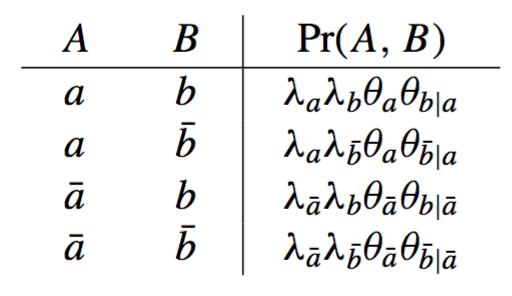
\includegraphics[width=0.35\textwidth]{figures/jpd_ind.png}
    \caption{The JPD from Figure \ref{fig:jpd} with indicator variables for each JPD variable.}
    \label{fig:jpd_ind}
    \end{center}
\end{figure}

In 2011, \cite{Poon2011} extended the idea of the polynomial network for any unnormalized distribution.
In practice, that means that any non-negative function can be represented as a polynomial network.
This extension is now known as \emph{sum-product networks} (SPNs).

One can draw the network polynomial as a directed acyclic graph (DAG).
Here, each multiplication is represented by a multiplication node, where the children are the factors involved in that particular multiplication.
Sum nodes represent summing terms of the polynomial.
The polynomial is written in a way that allows a pattern to form in the correspondent DAG.
This pattern is a layer of sum and a layer of product.
Thus, the name of the model SPNs.

\begin{example}
The JPD in Figure \ref{fig:jpd_ind} has a network polynomial described in Equation (\ref{eq:np}).
This network polynomial can be draw as a DAG, as illustrated in Figure \ref{fig:spn}.
Notice that multiplications in (\ref{eq:np}) are represented as a multiplication node in Figure \ref{fig:spn} where the children are the involved factors.
Similarly, sum in (\ref{eq:np}) are shown as sum nodes in Figure \ref{fig:spn}.t
\end{example}

\begin{figure}[hbt]
    \begin{center}
    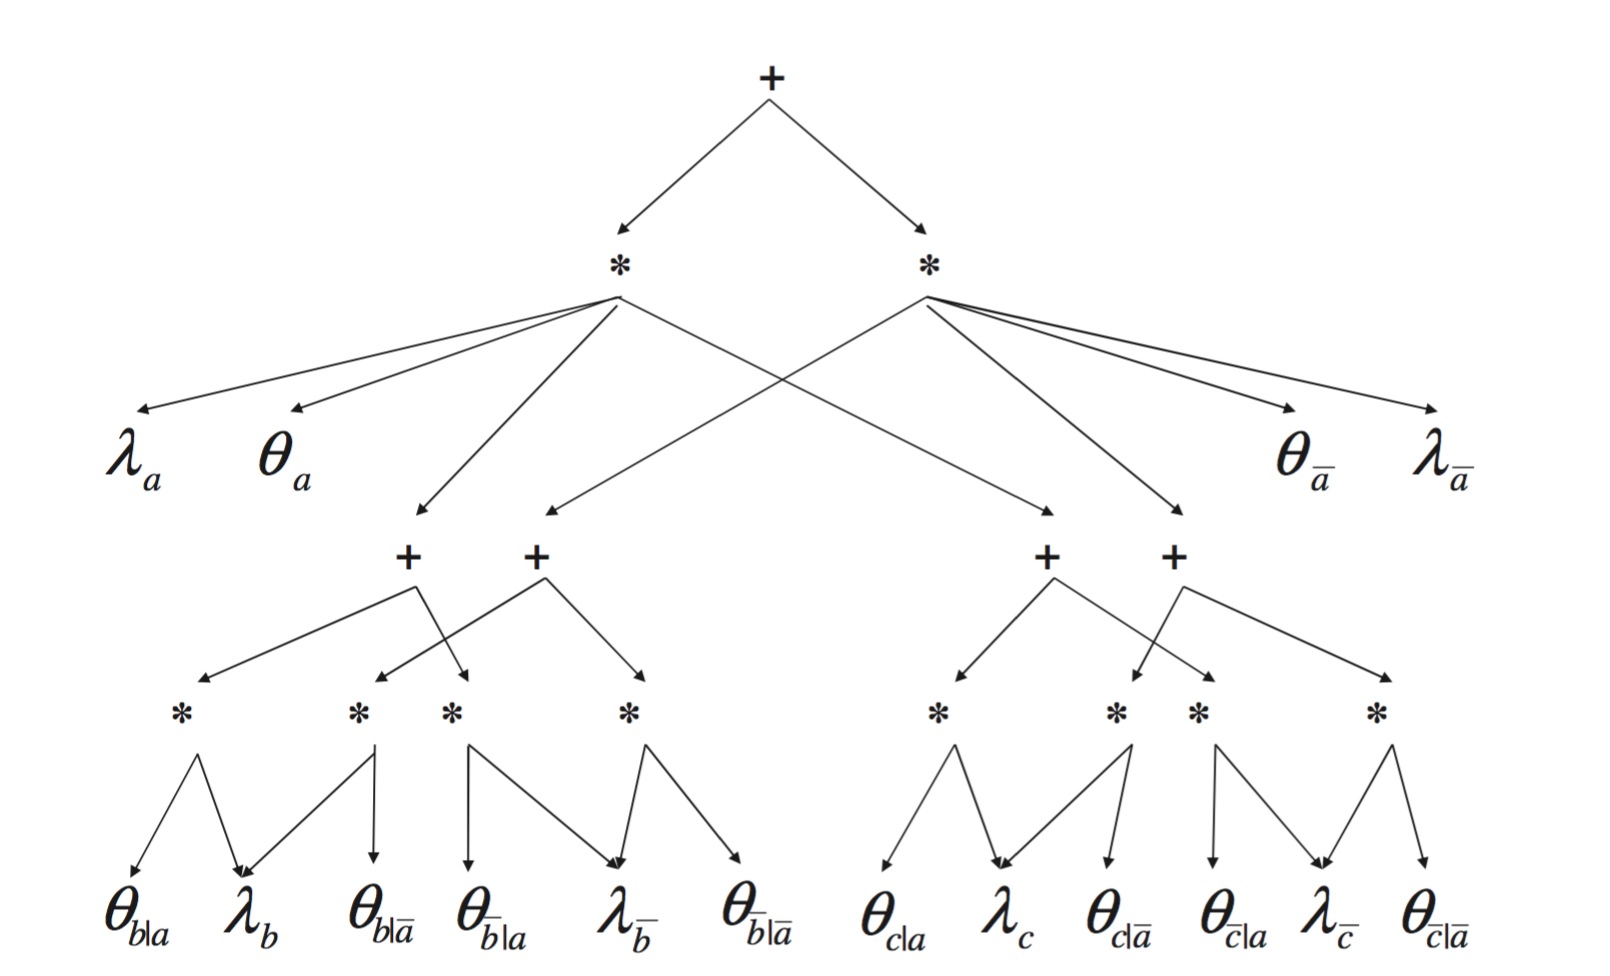
\includegraphics[width=\textwidth]{figures/spn.png}
    \caption{A SPN representing the JPD in Figure \ref{fig:jpd_ind}.}
    \label{fig:spn}
    \end{center}
\end{figure}

Inference in these models can be done by propagating up and down in the SPN DAG, as proposed by the \emph{differential method} \cite{Darwiche:2003hx}.
It is out of the scope of this paper to explain the differential approach when computing marginals for all variables of the JPD.
But it is of our interest the process of propagation itself.
Consider, for instance, propagating up in the DAG.
Values for each node are computed by following the operators.
Notice that nodes in the same layer can be computed simultaneously, since one does not require the value from the other.

\begin{example}
    Consider the SPN in Figure \ref{fig:spn}.
    When propagating up in this DAG, the first product layer is computed.
    Here, $\theta_{b|a}$ is multiplied with $\lambda_b$, for instance.
    But notice that $\lambda_b$ can also be multiplied with $\theta_{b|\overline{a}}$, simultaneously.
\end{example}

This paper proposes a method for parallelizing the computation at each layer of the SPN, as described in the next section.
